\documentclass[conference,onecolumn,12pt]{IEEEtran}
\IEEEoverridecommandlockouts
\hyphenation{op-tical net-works semi-conduc-tor}
\usepackage{fancyhdr}
\usepackage{lipsum}
\usepackage{amsmath,amssymb,amsfonts}
\usepackage{algorithmic}
\usepackage{graphicx}
\usepackage{textcomp}
\usepackage{comment}
\usepackage{xcolor}
\usepackage{float}
\usepackage{svg}
\usepackage{tabularx}
\usepackage{hyperref}
\usepackage{breqn}
\usepackage{makecell}
\usepackage{siunitx}
\usepackage{hyperref}
\usepackage{multirow}
\usepackage{booktabs}
\usepackage{stfloats}
\usepackage{titlesec}

\usepackage{listings}

\usepackage[T1]{fontenc}
\usepackage[utf8]{inputenc}
\usepackage[spanish,es-tabla]{babel}

\usepackage{longtable}


\lstset{
  basicstyle=\ttfamily\footnotesize,
  keywordstyle=\color{blue},
  commentstyle=\color{gray},
  stringstyle=\color{orange},
  numbers=left,
  numberstyle=\tiny\color{gray},
  backgroundcolor=\color{gray!10},
  frame=single,
  breaklines=true,
  captionpos=b
}
\selectlanguage{spanish}

\usepackage[style=numeric]{biblatex}  % Choose a style like numeric, authoryear, etc.
\addbibresource{references.bib}       % Note: use this instead of \bibliography

\defbibheading{bibliography}[\bibname]{\section*{Referencias}}

%\usepackage{circuitikz}

%\addbibresource{references.bib}
\renewcommand{\IEEEkeywordsname}{Palabras Clave}
\renewcommand{\tablename}{Tabla} 
\renewcommand{\abstractname}{Resumen} 
\renewcommand{\figurename}{Fig.}
\numberwithin{equation}{subsection}


%-------------------------No tocar de aqui para atras-----------

%-------------------------Título y nombres-----------
\begin{document}

\title{Tarea 2. Teoría de la información: \\Códigos de Huffman}
\author{
\IEEEauthorblockN{
Fabián Alonso Gómez Quesada\IEEEauthorrefmark{1}, Wilberth Daniel Gutiérrez Montero\IEEEauthorrefmark{2} \\
Nagel Eduardo Mejía Segura\IEEEauthorrefmark{3}, Oscar Mario González Cambronero\IEEEauthorrefmark{4}
}
\IEEEauthorblockA{
\IEEEauthorrefmark{1}\IEEEauthorrefmark{2}\IEEEauthorrefmark{3}\IEEEauthorrefmark{4} Escuela de Ingeniería en Electrónica, Instituto Tecnológico de Costa Rica. \\
\small Emails: fabi.goque@estudiantec.cr, wil.gutierrez@estudiantec.cr,\\ nagelmese@estudiantec.cr, oscargonzalezc@estudiantec.cr
}
}


\maketitle
\thispagestyle{plain}
\pagestyle{plain}
%------- %-------------------------Inicio----------- 

\begin{abstract} 

El presente informe expone la aplicación de los códigos de Huffman dentro del marco de la teoría de la información, a través de una serie de experimentos con códigos de programación junto a archivos de texto e imagen, con el fin de explorar conceptos como entropía, eficiencia de codificación, compresión sin pérdida y reconstrucción de datos. El lenguaje utilizado para el experimento es Python, que permite implementar el algoritmo de Huffman, calcular métricas estadísticas y comparar la codificación original del archivo con codificación generada.

\end{abstract} 
%-------------------------Palabras clave-----------
\begin{IEEEkeywords} Codificación, entropía, Huffman, Python.
\end{IEEEkeywords} 

\section{Introducción}

La teoría de la información constituye una base fundamental en el estudio de sistemas de comunicación. Dentro de este campo, los códigos de Huffman se destacan como una técnica eficiente para la compresión sin pérdida de datos, eliminando redundancias presentes en las fuentes de información. El objetivo del presente informe es explorar de manera práctica los conceptos relacionados con la entropía, la codificación eficiente y la reconstrucción de datos utilizando códigos de Huffman. A partir de la implementación en Python de dicho algoritmo, se analizará su rendimiento sobre distintos tipos de datos, se evaluará la eficiencia comparada con la codificación original, y se examinará cómo la entropía de una fuente afecta la compresibilidad de sus datos. 





\section{Desarrollo del proyecto}

\subsection{Algoritmo de Huffman}

\textbf{¿Cómo se implementa el algoritmo de generación de códigos Huffman?}


El script “huffman base.py” comienza recibiendo instrucciones desde la línea de comandos a través de la función myfunc(argv), la cual se encarga de interpretar los argumentos para identificar el archivo de entrada, cuya ruta debe ser proporcionada por el usuario. A continuación, se definen las rutas y nombres para los archivos: comprimido, diccionario y descomprimido. Posteriormente, el archivo original sin comprimir se lee byte por byte en modo binario y su contenido se almacena en una cadena de texto. Seguidamente, se implementan funciones relacionadas con la creación y manipulación del árbol binario utilizado en el proceso de compresión de Huffman. Una vez construido el árbol y sus nodos, se recorre para asignar un código binario a cada símbolo, el cual se guarda en un diccionario que enlaza símbolos con sus respectivos códigos.
\\
\\
\textbf{¿Cómo están codificados los datos del archivo solo\textunderscore abc\textunderscore cien.txt? ¿Cuántos bits se usan para representar cada carácter? ¿Qué espera observar al correr el algoritmo de Huffman?}

El archivo de prueba solo_abc_cien.txt contiene múltiples repeticiones de las letras de la “A” a la “Z”, específicamente 100 veces cada una, lo que hace que todos los símbolos tengan una probabilidad de aparición similar. Los datos están codificados en formato ASCII bajo el estándar UTF-8, lo cual implica que cada carácter ocupa 8 bits. Aunque UTF-8 permite longitudes variables por carácter, en este caso se emplea una codificación fija de 1 byte (8 bits) por símbolo. Al aplicar el algoritmo de Huffman sobre este archivo, se espera que los caracteres más frecuentes se codifiquen con menos bits; sin embargo, dado que todos los símbolos tienen la misma frecuencia, es razonable anticipar que las longitudes de los códigos resultantes sean muy similares entre sí. En consecuencia, la varianza del código generado será baja y el diccionario Huffman mostrará una tabla donde cada símbolo estará asociado a un código binario de longitud comparable.
\\
\\
\textbf{¿Cuáles son sus observaciones al ejecutar el código sobre el archivo llamado solo\textunderscore abc\textunderscore cien.txt?}

Al correr el código con dicho archivo, se obtiene la Tabla \ref{tab:huffman_abc} donde se observa que la mayoría de códigos tienen 5 bits, con excepción de 6 simbolos que contemplan 4 bits.

\begin{table}[h!]
    \centering
    \caption{Códigos Huffman para caracteres ASCII (A-Z)}
    \label{tab:huffman_abc}
    \begin{tabular}{ccc}
    \toprule
    \textbf{Char (decimal)} & \textbf{Símbolo} & \textbf{Código Huffman} \\
    \midrule
    65 & A & 0001 \\
    66 & B & 0000 \\
    67 & C & 0011 \\
    68 & D & 0010 \\
    69 & E & 10101 \\
    70 & F & 10100 \\
    71 & G & 10111 \\
    72 & H & 10110 \\
    73 & I & 10001 \\
    74 & J & 10000 \\
    75 & K & 10011 \\
    76 & L & 10010 \\
    77 & M & 11101 \\
    78 & N & 11100 \\
    79 & O & 11111 \\
    80 & P & 11110 \\
    81 & Q & 11001 \\
    82 & R & 11000 \\
    83 & S & 11011 \\
    84 & T & 11010 \\
    85 & U & 01101 \\
    86 & V & 01100 \\
    87 & W & 01111 \\
    88 & X & 01110 \\
    89 & Y & 0101 \\
    90 & Z & 0100 \\
    \bottomrule
    \end{tabular}
\end{table}

Las hipótesis sobre el comportamiento de los archivos con el código de Huffman:

\begin{itemize}
    \item \textbf{todo\_ascii\_cien.bin}: El archivo consiste de los 256 códigos para ASCII repetidos 100 veces, por lo tanto, cada simbolo es equiprobable, la entropía sería igual a $\log_2(8)$, si bien los códigos van a cambiar por como está programado el código de huffman, sin embargo, la longitud del código se mantiene en 8 bits. La eficiencia no cambia con el código nuevo.
    \item \textbf{shannon\_intro.txt}: El archivo contiene texto relacionado con los fundamentos teóricos de la comunicación, posiblemente basado en los trabajos de teoría de Claude Shannon. En él se aborda cómo cuantificar la información transmitida en un sistema de comunicación y cómo diferentes esquemas de modulación, como PCM (modulación por pulsos codificados) y PPM (modulación por posición de pulsos), logran intercambiar ancho de banda por mejoras en la relación señal/ruido. Al aplicar el algoritmo de Huffman sobre este archivo, se espera que se asignen códigos de longitud variable a los caracteres, donde aquellos que aparecen con mayor frecuencia reciban códigos más cortos. Esto se traduce en una codificación más eficiente al reducir la longitud promedio del código.
    \item \textbf{h\_cero.bin}: El archivo contiene exclusivamente la letra "H" repetida a lo largo de todo el archivo. Al tratarse de una fuente con un único símbolo, la entropía es mínima (cero en teoría), y el código de Huffman asignado será extremadamente simple: bastará con un solo bit para representar toda la información. En este caso, la longitud promedio del código también será mínima y la eficiencia será del 100%, ya que no existe redundancia adicional que pueda ser explotada.
    \item \textbf{4.1.01.tiff}: Es una imagen, que muestra una persona con vestimenta y un fondo con gran variedad de colores, lo que implica una alta diversidad de valores de píxeles. Desde el punto de vista de la teoría de la información, esto se traduce en una alta entropía, ya que hay poca redundancia en los datos. Al aplicar Huffman, la longitud promedio del código tenderá a ser mayor, ya que los símbolos tienen probabilidades más uniformes y se requiere más información para representarlos. En consecuencia, la eficiencia de compresión será menor comparada con imágenes más simples o menos variadas, ya que hay menos redundancia que explotar.
    \item \textbf{4.2.03.tiff}: Es una imagen, que muestra un mandril con gran variedad de colores, lo que implica una alta diversidad de valores de píxeles. Desde el punto de vista de la teoría de la información, esto se traduce en una alta entropía, ya que hay poca redundancia en los datos. Al aplicar Huffman, la longitud promedio del código tenderá a ser mayor, ya que los símbolos tienen probabilidades más uniformes y se requiere más información para representarlos. En consecuencia, la eficiencia de compresión será menor comparada con imágenes más simples o menos variadas, ya que hay menos redundancia que explotar.
    \item \textbf{5.1.11.tiff}: Es una imagen, que muestra un avión en escala de grises, lo que reduce considerablemente la cantidad de colores posibles. Esto puede generar mayor redundancia en los datos, por tanto, la entropía es moderada, y el algoritmo de Huffman puede asignar códigos más cortos a los valores de gris más frecuentes. Se espera una longitud promedio del código menor que en imágenes a color, y una eficiencia de codificación aceptable.
    \item \textbf{5.1.13.tiff}: Es una imagen, que muestra un fondo blanco con patrones de polígonos, números en negro y algunos grises. Debido a su simplicidad y contraste marcado entre pocos tonos, presenta una baja entropía, ya que la mayoría de los píxeles corresponden al fondo blanco. En este escenario, Huffman puede asignar códigos muy cortos a los símbolos más comunes, como el blanco, y más largos a los símbolos menos frecuentes. Esto se traduce en una longitud de código promedio baja y una alta eficiencia de compresión, ya que el algoritmo aprovecha al máximo la redundancia presente.
    \item \textbf{7.1.02.tiff}: Es una imagen, que muestra en escala de grises un jet en tierra, donde la reducción en la paleta de colores disminuye la entropía respecto a una imagen a color. La longitud promedio del código depende de la distribución de tonos, pero se espera moderada, y la eficiencia se espera sea buena ya que predominan algunos tonos de grises en grandes áreas.
\end{itemize}

Se realizó la modificación al script para obtener algunos parámetros como la entropía, la longitud media, varianza, eficiencia de la codificación original y eficiencia del nuevo código generado. En la Fig. \ref{listing1} se observa la modificación al script para el cálculo de los parámetros requeridos.

%//*\begin{figure}[!h]
 %   \begin{center}
%        \includegraphics[width=0.9\linewidth]%{figures/modscript.png}
 %       \caption{Modificación del script para el cálculo de nuevos parámetros}
   %     \label{fig:modscript}
  %  \end{center}
%%\end{figure}
%%

\begin{lstlisting}[language=Python, caption={Modificación del script para el cálculo de nuevos parámetros}, label={listing1}]

#Determinar e imprimir la entropia de la fuente:
information= lambda p:p*log2(1/p)
entropy=0
for code in freq:
    entropy+=information(freq[code])
print("Entropia de la Fuente: " + str(entropy))

#Determinar e imprimir el largo promedio de los codigos:
avg_length_new=0
for code in huffmanCode:
   avg_length_new+=len(huffmanCode[code])*freq[code]
print("Largo promedio: " + str(avg_length_new))

#Determinar e imprimir la varianza del nuevo codigo generado:
code_variance_new=0
for code in huffmanCode:
    code_variance_new+=freq[code]*((len(huffmanCode[code])-avg_length_new)**2)
print("Varianza del codigo original: " + str(code_variance_new))

#Determinar e imprimir la eficiencia del codigo original:
avg_length_old=entropy/8 #hardcoded a 8 bits en las codificaciones originales
print("Eficiencia del codigo original: " + str(avg_length_old))

#Determinar e imprimir la eficiencia del nuevo codigo generado:
try:
    new_code_efficiency=entropy/avg_length_new
    print("Eficiencia del nuevo codigo generado: " + str(new_code_efficiency))
except:
    print("Largo promedio igual a 0, todos los simbolos son iguales y no se genera diccionario de compresion.")

\end{lstlisting}


En la Tabla \ref{tab:huffman_resultados} se observan los resultados al ejecutar el script con todos los archivos mostrados.

\hfill\break \hfill\break \hfill\break \hfill\break \hfill\break
\hfill\break \hfill\break 


 \begin{table*}[h!]
    \centering
    \caption{Resultados de codificación Huffman sobre distintos archivos.}
    \label{tab:huffman_resultados}
    \begin{tabular}{lccccc}
    \toprule
    \textbf{Archivo} & \textbf{Entropía} & \textbf{Largo Promedio} & \textbf{Varianza} & \textbf{Efic. Código Orig.} & \textbf{Efic. Código Gen.} \\
    \midrule
    todo\_ascii\_cien.bin & 8.00 & 8.00 & 3.16e-30 & 1.00 & 1.00 \\
    shannon\_intro.txt & 4.37 & 4.40 & 2.08 & 0.55 & 0.99 \\
    h\_cero.bin & 0.00 & 0.00 & 0.00 & 0.00 & - \\
    4.1.01.tiff & 6.90 & 6.93 & 1.01 & 0.863 & 0.996 \\
    4.2.03.tiff & 7.76 & 7.80 & 0.607 & 0.970 & 0.995 \\
    5.1.11.tiff & 6.46 & 6.48 & 2.27 & 0.808 & 0.997 \\
    5.1.13.tiff & 1.57 & 1.95 & 6.32 & 0.196 & 0.803 \\
    7.1.02.tiff & 4.01 & 4.06 & 3.68 & 0.501 & 0.989 \\
    \bottomrule
    \end{tabular}
\end{table*}

\begin{itemize}
    \item \textbf{todo\_ascii\_cien.bin}: En este caso se observa que la entropía y la longitud promedio son de exactamente 8 bits, lo que se alinea con una codificación ASCII de 256 símbolos equiprobables, la eficiencia original y generada son ambas de 1, lo que es coherente ya que no hay redundancia que comprimir.
    
    \begin{table}[h!]
\centering
\caption{Código Huffman para todo\_ascii\_cien.bin}
\label{tab:huffman_todo_ascii}
\begin{tabular}{cccccccccccc}
\toprule
\textbf{Char} & \textbf{Código} & \textbf{Char} & \textbf{Código} & \textbf{Char} & \textbf{Código} & \textbf{Char} & \textbf{Código} & \textbf{Char} & \textbf{Código} & \textbf{Char} & \textbf{Código} \\
\midrule
0 & 10101010 & 43 & 10000001 & 86 & 11111100 & 129 & 00101011 & 172 & 00000110 & 215 & 01111101 \\
1 & 10101011 & 44 & 10000110 & 87 & 11111101 & 130 & 00101000 & 173 & 00000111 & 216 & 01110010 \\
2 & 10101000 & 45 & 10000111 & 88 & 11110010 & 131 & 00101001 & 174 & 00000100 & 217 & 01110011 \\
3 & 10101001 & 46 & 10000100 & 89 & 11110011 & 132 & 00101110 & 175 & 00000101 & 218 & 01110000 \\
4 & 10101110 & 47 & 10000101 & 90 & 11110000 & 133 & 00101111 & 176 & 00011010 & 219 & 01110001 \\
5 & 10101111 & 48 & 10011010 & 91 & 11110001 & 134 & 00101100 & 177 & 00011011 & 220 & 01110110 \\
6 & 10101100 & 49 & 10011011 & 92 & 11110110 & 135 & 00101101 & 178 & 00011000 & 221 & 01110111 \\
7 & 10101101 & 50 & 10011000 & 93 & 11110111 & 136 & 00100010 & 179 & 00011001 & 222 & 01110100 \\
8 & 10100010 & 51 & 10011001 & 94 & 11110100 & 137 & 00100011 & 180 & 00011110 & 223 & 01110101 \\
9 & 10100011 & 52 & 10011110 & 95 & 11110101 & 138 & 00100000 & 181 & 00011111 & 224 & 01001010 \\
10 & 10100000 & 53 & 10011111 & 96 & 11001010 & 139 & 00100001 & 182 & 00011100 & 225 & 01001011 \\
11 & 10100001 & 54 & 10011100 & 97 & 11001011 & 140 & 00100110 & 183 & 00011101 & 226 & 01001000 \\
12 & 10100110 & 55 & 10011101 & 98 & 11001000 & 141 & 00100111 & 184 & 00010010 & 227 & 01001001 \\
13 & 10100111 & 56 & 10010010 & 99 & 11001001 & 142 & 00100100 & 185 & 00010011 & 228 & 01001110 \\
14 & 10100100 & 57 & 10010011 & 100 & 11001110 & 143 & 00100101 & 186 & 00010000 & 229 & 01001111 \\
15 & 10100101 & 58 & 10010000 & 101 & 11001111 & 144 & 00111010 & 187 & 00010001 & 230 & 01001100 \\
16 & 10111010 & 59 & 10010001 & 102 & 11001100 & 145 & 00111011 & 188 & 00010110 & 231 & 01001101 \\
17 & 10111011 & 60 & 10010110 & 103 & 11001101 & 146 & 00111000 & 189 & 00010111 & 232 & 01000010 \\
18 & 10111000 & 61 & 10010111 & 104 & 11000010 & 147 & 00111001 & 190 & 00010100 & 233 & 01000011 \\
19 & 10111001 & 62 & 10010100 & 105 & 11000011 & 148 & 00111110 & 191 & 00010101 & 234 & 01000000 \\
20 & 10111110 & 63 & 10010101 & 106 & 11000000 & 149 & 00111111 & 192 & 01101010 & 235 & 01000001 \\
21 & 10111111 & 64 & 11101010 & 107 & 11000001 & 150 & 00111100 & 193 & 01101011 & 236 & 01000110 \\
22 & 10111100 & 65 & 11101011 & 108 & 11000110 & 151 & 00111101 & 194 & 01101000 & 237 & 01000111 \\
23 & 10111101 & 66 & 11101000 & 109 & 11000111 & 152 & 00110010 & 195 & 01101001 & 238 & 01000100 \\
24 & 10110010 & 67 & 11101001 & 110 & 11000100 & 153 & 00110011 & 196 & 01101110 & 239 & 01000101 \\
25 & 10110011 & 68 & 11101110 & 111 & 11000101 & 154 & 00110000 & 197 & 01101111 & 240 & 01011010 \\
26 & 10110000 & 69 & 11101111 & 112 & 11011010 & 155 & 00110001 & 198 & 01101100 & 241 & 01011011 \\
27 & 10110001 & 70 & 11101100 & 113 & 11011011 & 156 & 00110110 & 199 & 01101101 & 242 & 01011000 \\
28 & 10110110 & 71 & 11101101 & 114 & 11011000 & 157 & 00110111 & 200 & 01100010 & 243 & 01011001 \\
29 & 10110111 & 72 & 11100010 & 115 & 11011001 & 158 & 00110100 & 201 & 01100011 & 244 & 01011110 \\
30 & 10110100 & 73 & 11100011 & 116 & 11011110 & 159 & 00110101 & 202 & 01100000 & 245 & 01011111 \\
31 & 10110101 & 74 & 11100000 & 117 & 11011111 & 160 & 00001010 & 203 & 01100001 & 246 & 01011100 \\
32 & 10001010 & 75 & 11100001 & 118 & 11011100 & 161 & 00001011 & 204 & 01100110 & 247 & 01011101 \\
33 & 10001011 & 76 & 11100110 & 119 & 11011101 & 162 & 00001000 & 205 & 01100111 & 248 & 01010010 \\
34 & 10001000 & 77 & 11100111 & 120 & 11010010 & 163 & 00001001 & 206 & 01100100 & 249 & 01010011 \\
35 & 10001001 & 78 & 11100100 & 121 & 11010011 & 164 & 00001110 & 207 & 01100101 & 250 & 01010000 \\
36 & 10001110 & 79 & 11100101 & 122 & 11010000 & 165 & 00001111 & 208 & 01111010 & 251 & 01010001 \\
37 & 10001111 & 80 & 11111010 & 123 & 11010001 & 166 & 00001100 & 209 & 01111011 & 252 & 01010110 \\
38 & 10001100 & 81 & 11111011 & 124 & 11010110 & 167 & 00001101 & 210 & 01111000 & 253 & 01010111 \\
39 & 10001101 & 82 & 11111000 & 125 & 11010111 & 168 & 00000010 & 211 & 01111001 & 254 & 01010100 \\
40 & 10000010 & 83 & 11111001 & 126 & 11010100 & 169 & 00000011 & 212 & 01111110 & 255 & 01010101 \\
41 & 10000011 & 84 & 11111110 & 127 & 11010101 & 170 & 00000000 & 213 & 01111111 \\
42 & 10000000 & 85 & 11111111 & 128 & 00101010 & 171 & 00000001 & 214 & 01111100 \\
\bottomrule
\end{tabular}
\end{table}
    
    \item \textbf{shannon\_intro.txt}: La entropía indica una fuente con distribución de símbolos desigual, pero al ser la longitud promedio muy cercana a la entropía, sugiere que la codificación fue eficiente. La varianza muestra una distribución dispersa de las longitudes del código, lo cual es consistente con un texto donde caracteres como espacios o vocales son más frecuentes. La eficiencia original y la del código generado evidencian que hay una mejora significativa al utilizar Huffman.
    
\begin{table}[H]
\centering
\caption{Código Huffman para shannon\_intro.txt}
\label{tab:huffman_shannon}
\begin{tabular}{cccccccccccc}
\toprule
\textbf{Char} & \textbf{Código} & \textbf{Char} & \textbf{Código} & \textbf{Char} & \textbf{Código} & \textbf{Char} & \textbf{Código} & \textbf{Char} & \textbf{Código} & \textbf{Char} & \textbf{Código} \\
\midrule
32 & 111 & 108 & 10001 & 118 & 0100100 & 65 & 010010110 & 67 & 01001011111 & 47 & 100001111001 \\
101 & 001 & 109 & 01000 & 44 & 0001101 & 49 & 000110011 & 45 & 01001011110 & 66 & 100001111000 \\
116 & 1100 & 100 & 00010 & 120 & 00011000 & 50 & 000110010 & 58 & 11010000001 & 156 & 100001111011 \\
105 & 1011 & 117 & 00001 & 13 & 00000010 & 107 & 000000110 & 87 & 11010000000 & 157 & 100001111010 \\
115 & 1001 & 102 & 110101 & 10 & 00000001 & 226 & 000000001 & 48 & 11010000011 & 86 & 110100000101 \\
111 & 0111 & 103 & 100000 & 84 & 110100011 & 128 & 000000000 & 70 & 01001011100 & 68 & 000000111010 \\
110 & 0110 & 112 & 010011 & 40 & 110100010 & 77 & 1000011111 & 122 & 01001010101 & 79 & 0000001110111 \\
97 & 0101 & 121 & 000111 & 41 & 110100001 & 80 & 0100101001 & 61 & 01001010100 & 74 & 0000001110110 \\
114 & 11011 & 98 & 000001 & 113 & 100001110 & 78 & 0100101000 & 72 & 00000011100 & 52 & 1101000001001 \\
104 & 10101 & 46 & 1101001 & 73 & 100001101 & 51 & 0100101011 & 106 & 010010111011 & 53 & 1101000001000 \\
99 & 10100 & 119 & 1000010 & 59 & 100001100 & 148 & 0000001111 & 83 & 010010111010 \\
\bottomrule
\end{tabular}
\end{table}
    
    \item \textbf{h\_cero.bin}: Al contener un único símbolo, se esperaba y se obtuvo una entropía de 0, al igual que la longitud del código. La eficiencia del código original es 0, porque usar más de un bit para un símbolo único es completamente redundante. No se reporta eficiencia generada porque no hay nada que codificar.  
    
\begin{table}[H]
\centering
\caption{Código Huffman para h\_cero.bin}
\label{tab:huffman_cerobin}
\begin{tabular}{cc}
\toprule
\textbf{Char} & \textbf{Código} \\
\midrule
72   &  \\     
\bottomrule
\end{tabular}
\end{table}
    
    \item \textbf{4.1.01.tiff}: La imagen tiene entropía moderadamente alta y longitud promedio muy cercana a la entropía. La eficiencia del código generado es casi 1, indicando que Huffman está aprovechando bien las frecuencias relativas.
    
    \begin{table}[H]
\centering
\caption{Código Huffman para 4.1.01.tiff}
\label{tab:huffman_4.1.01.tiff}
\begin{tabular}{cccccccccccc}
\toprule
\textbf{Char} & \textbf{Código} & \textbf{Char} & \textbf{Código} & \textbf{Char} & \textbf{Código} & \textbf{Char} & \textbf{Código} & \textbf{Char} & \textbf{Código} & \textbf{Char} & \textbf{Código} \\
\midrule
44 & 111000 & 39 & 1111000 & 45 & 0110111 & 126 & 10010110 & 116 & 011001101 & 0 & 01100111001 \\
42 & 110101 & 18 & 1110110 & 68 & 0110110 & 132 & 01110100 & 164 & 011001100 & 165 & 01100111000 \\
46 & 110011 & 30 & 1110101 & 41 & 0110101 & 77 & 01010001 & 111 & 010101111 & 177 & 00110111000 \\
49 & 110000 & 16 & 1110100 & 105 & 0110100 & 75 & 01010000 & 120 & 010101110 & 185 & 00001001001 \\
40 & 101110 & 14 & 1110011 & 27 & 0110010 & 67 & 00110110 & 142 & 010101101 & 190 & 111011100101 \\
52 & 101000 & 55 & 1110010 & 103 & 0110001 & 90 & 00110101 & 161 & 010101100 & 226 & 110010011101 \\
38 & 100100 & 8 & 1101110 & 108 & 0110000 & 71 & 00011111 & 119 & 001101111 & 168 & 110010011100 \\
37 & 100010 & 20 & 1101101 & 17 & 0101010 & 149 & 00011110 & 122 & 001101001 & 197 & 100110101100 \\
1 & 100001 & 100 & 1101001 & 110 & 0101001 & 102 & 00011101 & 170 & 001101000 & 193 & 100110101001 \\
4 & 011110 & 64 & 1101000 & 123 & 0100101 & 53 & 00011100 & 167 & 000010011 & 229 & 001101110011 \\
3 & 011100 & 13 & 1100101 & 22 & 0100100 & 140 & 00001011 & 148 & 1111110001 & 233 & 001101110010 \\
34 & 010111 & 29 & 1100011 & 48 & 0100001 & 97 & 00001010 & 151 & 1101100111 & 211 & 000010010001 \\
2 & 010110 & 9 & 1100010 & 26 & 0100000 & 96 & 00001000 & 173 & 1101100110 & 207 & 000010010000 \\
47 & 010011 & 10 & 1011111 & 134 & 0011111 & 152 & 111111011 & 180 & 1100100110 & 200 & 1110111001001 \\
50 & 010001 & 62 & 1011110 & 70 & 0011110 & 69 & 111111010 & 154 & 1010101111 & 204 & 1110111001000 \\
35 & 001110 & 12 & 1011011 & 66 & 0010011 & 56 & 111111001 & 183 & 1010101110 & 172 & 1001101011010 \\
7 & 001100 & 28 & 1011001 & 115 & 0010010 & 107 & 111011101 & 157 & 0011011101 & 175 & 1001101010001 \\
32 & 001011 & 15 & 1010110 & 137 & 0000001 & 58 & 110111111 & 196 & 0000100101 & 179 & 1001101010000 \\
57 & 001010 & 11 & 1010100 & 21 & 0000000 & 65 & 110111110 & 176 & 11111100001 & 218 & 0110011101011 \\
5 & 001000 & 59 & 1010011 & 51 & 11101111 & 155 & 110110010 & 186 & 11111100000 & 236 & 0110011101010 \\
54 & 000110 & 23 & 1001111 & 24 & 11011110 & 131 & 110010010 & 192 & 11101110011 & 215 & 0110011101000 \\
88 & 000101 & 76 & 1001110 & 113 & 11011000 & 112 & 101101001 & 189 & 11101110001 & 182 & 10011010110110 \\
84 & 000100 & 60 & 1001100 & 36 & 11001000 & 158 & 101011111 & 206 & 11101110000 & 240 & 01100111010011 \\
80 & 000011 & 91 & 1001010 & 121 & 10110101 & 61 & 101011110 & 202 & 11001001111 & 203 & 100110101101110 \\
43 & 000001 & 33 & 1000111 & 118 & 10110001 & 106 & 101010110 & 216 & 10110100011 & 254 & 011001110100100 \\
82 & 1111111 & 78 & 1000110 & 128 & 10110000 & 136 & 101001001 & 209 & 10110100010 & 250 & 1001101011011111 \\
6 & 1111101 & 25 & 1000001 & 139 & 10101110 & 130 & 101001000 & 199 & 10110100001 & 247 & 1001101011011110 \\
93 & 1111100 & 95 & 1000000 & 143 & 10101010 & 117 & 100110100 & 162 & 10110100000 & 243 & 0110011101001011 \\
86 & 1111011 & 19 & 0111111 & 125 & 10100101 & 133 & 011101011 & 222 & 10011010111 & 237 & 01100111010010101 \\
31 & 1111010 & 98 & 0111110 & 129 & 10011011 & 114 & 011101010 & 212 & 10011010101 & 230 & 01100111010010100 \\
72 & 1111001 & 74 & 0111011 & 146 & 10010111 & 145 & 011001111 & 219 & 01100111011 \\
\bottomrule
\end{tabular}
\end{table}
    
    \item \textbf{4.2.03.tiff}: Presenta una entropía y longitud promedio muy similar, como era de esperarse para una imagen con gran variabilidad de colores. La eficiencia del código generado es alta, aunque la eficiencia original también es bastante buena, reflejando que el archivo original ya está optimizado.
    
    \begin{table}[H]
\centering
\caption{Código Huffman para 4.2.03.tiff}
\label{tab:huffman_4.2.03.tiff}
\begin{tabular}{cccccccccccc}
\toprule
\textbf{Char} & \textbf{Código} & \textbf{Char} & \textbf{Código} & \textbf{Char} & \textbf{Código} & \textbf{Char} & \textbf{Código} & \textbf{Char} & \textbf{Código} & \textbf{Char} & \textbf{Código} \\
\midrule
88 & 1000000 & 111 & 0010010 & 144 & 11100000 & 174 & 10101100 & 222 & 110110010 & 212 & 010110010 \\
76 & 0111111 & 98 & 0010001 & 145 & 11011111 & 177 & 10101011 & 228 & 110101101 & 30 & 001011011 \\
79 & 0111110 & 124 & 0010000 & 141 & 11011110 & 164 & 10101001 & 205 & 110101100 & 29 & 000101011 \\
83 & 0111101 & 121 & 0001111 & 159 & 11011101 & 181 & 10101000 & 239 & 110100011 & 28 & 000101010 \\
92 & 0111011 & 67 & 0001110 & 190 & 11011100 & 162 & 10100111 & 221 & 110001011 & 247 & 1111011111 \\
81 & 0111010 & 101 & 0001101 & 60 & 11011011 & 173 & 10100110 & 223 & 110001010 & 27 & 1111011110 \\
96 & 0111001 & 109 & 0001100 & 188 & 11011010 & 183 & 10100100 & 226 & 110000001 & 26 & 1101000101 \\
91 & 0111000 & 68 & 0001011 & 61 & 11011000 & 171 & 10100011 & 225 & 110000000 & 248 & 1011000111 \\
73 & 0110111 & 106 & 0001001 & 149 & 11010111 & 165 & 10100010 & 238 & 101111011 & 25 & 1011000110 \\
86 & 0110110 & 114 & 0001000 & 191 & 11010101 & 170 & 10100001 & 37 & 101111010 & 23 & 1001110111 \\
89 & 0110101 & 123 & 0000111 & 187 & 11010100 & 55 & 10100000 & 227 & 101110011 & 24 & 1001110110 \\
75 & 0110100 & 116 & 0000110 & 146 & 11010011 & 54 & 10011111 & 220 & 101110010 & 22 & 1001000110 \\
112 & 0110011 & 65 & 0000101 & 189 & 11010010 & 198 & 10011110 & 230 & 101100010 & 21 & 1000100001 \\
78 & 0110010 & 117 & 0000100 & 148 & 11010000 & 53 & 10011100 & 244 & 101011011 & 19 & 1000100000 \\
94 & 0110001 & 131 & 0000011 & 150 & 11001111 & 178 & 10011011 & 206 & 101011010 & 249 & 1000010010 \\
99 & 0110000 & 63 & 0000001 & 194 & 11001110 & 180 & 10011010 & 229 & 101010101 & 20 & 0101100111 \\
71 & 0101111 & 127 & 0000000 & 59 & 11001101 & 51 & 10011000 & 237 & 101010100 & 18 & 0010110100 \\
97 & 0101110 & 192 & 11111111 & 156 & 11001100 & 175 & 10010110 & 36 & 101001011 & 17 & 11101111111 \\
80 & 0101101 & 128 & 11111110 & 184 & 11001011 & 52 & 10010101 & 35 & 101001010 & 250 & 11101111101 \\
77 & 0101011 & 119 & 11111101 & 185 & 11001010 & 199 & 10010011 & 236 & 100111010 & 16 & 11010001001 \\
103 & 0101010 & 122 & 11111100 & 176 & 11001001 & 49 & 10010000 & 219 & 100110011 & 15 & 11010001000 \\
82 & 0101001 & 135 & 11111011 & 57 & 11001000 & 48 & 10001111 & 207 & 100110010 & 14 & 10010001110 \\
85 & 0101000 & 64 & 11111010 & 157 & 11000111 & 50 & 10001110 & 34 & 100101111 & 13 & 01011001101 \\
108 & 0100111 & 125 & 11111001 & 58 & 11000110 & 47 & 10001001 & 232 & 100101110 & 251 & 01011001100 \\
72 & 0100110 & 126 & 11111000 & 163 & 11000100 & 46 & 10000111 & 218 & 100101001 & 12 & 00101101010 \\
70 & 0100101 & 129 & 11110110 & 153 & 11000011 & 200 & 10000110 & 231 & 100101000 & 11 & 111011111101 \\
115 & 0100100 & 66 & 11110101 & 158 & 11000010 & 201 & 10000101 & 245 & 100100101 & 0 & 111011111100 \\
84 & 0100011 & 62 & 11110011 & 155 & 11000001 & 45 & 01111001 & 33 & 100100100 & 10 & 111011111001 \\
90 & 0100010 & 132 & 11110010 & 151 & 10111111 & 44 & 01111000 & 208 & 100100010 & 252 & 100100011110 \\
95 & 0100001 & 133 & 11110001 & 161 & 10111110 & 43 & 01011000 & 234 & 100011011 & 9 & 100001001111 \\
93 & 0100000 & 134 & 11110000 & 154 & 10111100 & 202 & 00101100 & 217 & 100011010 & 8 & 100001001101 \\
107 & 0011111 & 143 & 11101110 & 182 & 10111011 & 203 & 00010100 & 233 & 100011001 & 7 & 100001001100 \\
105 & 0011110 & 193 & 11101101 & 186 & 10111010 & 42 & 00000101 & 216 & 100011000 & 5 & 001011010111 \\
87 & 0011101 & 130 & 11101100 & 56 & 10111000 & 41 & 00000100 & 209 & 100010111 & 6 & 001011010110 \\
74 & 0011100 & 147 & 11101011 & 172 & 10110111 & 242 & 111101110 & 235 & 100010110 & 253 & 1110111110001 \\
100 & 0011011 & 139 & 11101001 & 179 & 10110110 & 224 & 111101001 & 32 & 100010101 & 4 & 1110111110000 \\
102 & 0011010 & 137 & 11101000 & 169 & 10110101 & 39 & 111101000 & 31 & 100010100 & 3 & 1001000111111 \\
110 & 0011001 & 140 & 11100111 & 196 & 10110100 & 40 & 111011110 & 246 & 100010001 & 2 & 1001000111110 \\
113 & 0011000 & 195 & 11100110 & 160 & 10110011 & 240 & 111010101 & 214 & 100001000 & 1 & 1000010011101 \\
120 & 0010111 & 142 & 11100101 & 167 & 10110010 & 204 & 111010100 & 215 & 100000111 & 254 & 10000100111001 \\
118 & 0010101 & 152 & 11100011 & 197 & 10110000 & 243 & 111001001 & 213 & 100000110 & 255 & 10000100111000 \\
104 & 0010100 & 136 & 11100010 & 166 & 10101111 & 241 & 111001000 & 210 & 100000101 \\
69 & 0010011 & 138 & 11100001 & 168 & 10101110 & 38 & 110110011 & 211 & 100000100 \\
\bottomrule
\end{tabular}
\end{table}
    
    \item \textbf{5.1.11.tiff}:  Presenta entropía moderada y longitud muy similar, con una varianza considerable, lo cual puede deberse a que ciertos tonos se repiten más que otros. La eficiencia generada es muy alta, mostrando un uso efectivo del algoritmo.
    
    \begin{table}[H]
\centering
\caption{Código Huffman para 5.1.11.tiff}
\label{tab:huffman_5.1.11.tiff}
\begin{tabular}{cccccccccccc}
\toprule
\textbf{Char} & \textbf{Código} & \textbf{Char} & \textbf{Código} & \textbf{Char} & \textbf{Código} & \textbf{Char} & \textbf{Código} & \textbf{Char} & \textbf{Código} & \textbf{Char} & \textbf{Código} \\
\midrule
224 & 1000 & 193 & 1110100 & 153 & 11011110 & 124 & 1111111111 & 81 & 101100110011 & 50 & 1101011011010 \\
225 & 0011 & 190 & 1101100 & 161 & 11011101 & 120 & 1111000011 & 63 & 101100110010 & 99 & 1110010100101 \\
223 & 01011 & 188 & 1101001 & 162 & 11011100 & 125 & 1110010111 & 85 & 110101100001 & 78 & 1110010100100 \\
226 & 01001 & 189 & 1101000 & 157 & 11011011 & 121 & 1110010101 & 61 & 110101100000 & 74 & 1110010100111 \\
222 & 111000 & 191 & 1100110 & 158 & 11011010 & 122 & 1101011010 & 101 & 101001100011 & 55 & 1101011001011 \\
205 & 110010 & 187 & 1011000 & 152 & 11010111 & 118 & 1011001101 & 51 & 101001100010 & 87 & 1101011001010 \\
206 & 110001 & 184 & 1010010 & 150 & 11010101 & 123 & 1010011011 & 92 & 101001100101 & 75 & 1101011011001 \\
208 & 110000 & 186 & 1001001 & 151 & 11010100 & 119 & 0010110111 & 59 & 101001100100 & 62 & 1101011011000 \\
207 & 101111 & 185 & 0111001 & 155 & 11001111 & 116 & 0010110110 & 88 & 101001100111 & 41 & 1010011010001 \\
204 & 101110 & 176 & 0111000 & 154 & 11001110 & 114 & 0001011111 & 95 & 101001100110 & 60 & 1010011010000 \\
209 & 101101 & 182 & 0101010 & 148 & 10110010 & 117 & 0000100110 & 89 & 101001100001 & 231 & 1010011010011 \\
200 & 101011 & 172 & 0010001 & 149 & 10100111 & 115 & 11100101100 & 77 & 010101110001 & 3 & 1010011010010 \\
203 & 101010 & 180 & 0010000 & 146 & 10010001 & 230 & 11010110111 & 48 & 010101110000 & 42 & 1010011000000 \\
213 & 101000 & 181 & 0001110 & 147 & 10010000 & 112 & 11010110011 & 98 & 010101110011 & 49 & 0010111011001 \\
214 & 100111 & 173 & 0001010 & 144 & 01010110 & 106 & 10100110101 & 69 & 010101110010 & 44 & 0010111011000 \\
212 & 100110 & 179 & 0001001 & 145 & 00101111 & 113 & 01010111011 & 71 & 001011101101 & 84 & 0010111010011 \\
211 & 100101 & 178 & 0001000 & 142 & 00101100 & 111 & 01010111010 & 82 & 001011101000 & 43 & 11111111101111 \\
216 & 011111 & 174 & 0000101 & 143 & 00011110 & 110 & 00101110111 & 90 & 000101111011 & 45 & 11100101001101 \\
221 & 011110 & 171 & 0000011 & 137 & 00010110 & 1 & 00101110101 & 80 & 000101111010 & 46 & 10100110000011 \\
202 & 011101 & 177 & 0000010 & 138 & 00001000 & 108 & 00010111100 & 97 & 000010011101 & 8 & 00101110100100 \\
201 & 011011 & 169 & 0000000 & 139 & 00000011 & 107 & 00001001011 & 79 & 000010011100 & 39 & 111111111011101 \\
210 & 011010 & 168 & 11111110 & 136 & 00000010 & 105 & 00001001010 & 54 & 000010011111 & 4 & 111111111011100 \\
220 & 011001 & 170 & 11111011 & 140 & 111111110 & 64 & 00001001001 & 100 & 000010011110 & 232 & 111001010011000 \\
217 & 011000 & 175 & 11111010 & 141 & 111110001 & 109 & 00001001000 & 93 & 1111111110110 & 40 & 1110010100110010 \\
219 & 010100 & 183 & 11111001 & 135 & 111110000 & 56 & 111111111000 & 52 & 1111111110011 & 36 & 11100101001100111 \\
218 & 010001 & 167 & 11110111 & 134 & 111100000 & 67 & 111100001000 & 68 & 1111111110010 & 38 & 11100101001100110 \\
215 & 010000 & 163 & 11110110 & 133 & 111001001 & 57 & 111001011011 & 73 & 1111111110101 & 10 & 1010011000001001 \\
198 & 001010 & 164 & 11110001 & 132 & 111001000 & 91 & 111001011010 & 70 & 1111111110100 & 254 & 1010011000001000 \\
199 & 001001 & 166 & 11101101 & 131 & 101100111 & 65 & 111001010001 & 83 & 1111000010011 & 2 & 1010011000001011 \\
227 & 000110 & 228 & 11101100 & 130 & 010101111 & 58 & 111001010000 & 72 & 1111000010010 & 6 & 1010011000001010 \\
197 & 000011 & 0 & 11101011 & 229 & 001011100 & 103 & 110101100100 & 53 & 1111000010101 & 17 & 0010111010010101 \\
196 & 1111110 & 165 & 11101010 & 128 & 001011010 & 66 & 110101100011 & 86 & 1111000010100 & 21 & 0010111010010100 \\
195 & 1111010 & 156 & 11100111 & 127 & 000111111 & 96 & 110101100010 & 76 & 1111000010111 & 23 & 0010111010010111 \\
192 & 1111001 & 160 & 11100110 & 126 & 000111110 & 104 & 101100110001 & 94 & 1111000010110 & 28 & 0010111010010110 \\
194 & 1110111 & 159 & 11011111 & 129 & 000101110 & 102 & 101100110000 & 47 & 1101011011011 \\
\bottomrule
\end{tabular}
\end{table}
    
    \item \textbf{5.1.13.tiff}: La entropía es muy baja, lo que concuerda con la gran cantidad de fondo blanco. La longitud del código no está tan cercana a la entropía, y la varianza es alta, probablemente porque algunos símbolos menos frecuentes recibieron códigos largos. La eficiencia generada es notablemente baja, pero esto es esperable dado el contraste fuerte entre frecuencias muy distintas y aún así es mejor que la eficiencia original.
    
    \begin{table}[H]
\centering
\caption{Código Huffman para 5.1.13.tiff}
\label{tab:huffman_5.1.13.tiff}
\begin{tabular}{cccccccccccc}
\toprule
\textbf{Char} & \textbf{Código} & \textbf{Char} & \textbf{Código} & \textbf{Char} & \textbf{Código} & \textbf{Char} & \textbf{Código} & \textbf{Char} & \textbf{Código} & \textbf{Char} & \textbf{Código} \\
\midrule
255 & 1 & 157 & 0111100011 & 235 & 0100111111 & 39 & 0011100101 & 170 & 01111010110 & 201 & 01110010001 \\
3 & 000 & 249 & 0111100010 & 246 & 0100111110 & 164 & 0011100100 & 173 & 01111011101 & 83 & 01110010000 \\
4 & 0110 & 231 & 0111100001 & 135 & 0100110010 & 82 & 0011010101 & 68 & 01111011100 & 104 & 01110010011 \\
6 & 010010 & 245 & 0111001011 & 165 & 0100011001 & 77 & 0011010100 & 192 & 01111011111 & 125 & 01110010010 \\
5 & 001111 & 228 & 0111001010 & 206 & 0100011000 & 114 & 0011010001 & 127 & 01111011110 & 90 & 01110001101 \\
7 & 001100 & 191 & 0111000010 & 210 & 0100011011 & 176 & 0011010000 & 197 & 01111011001 & 171 & 01110001100 \\
8 & 001010 & 248 & 0101110111 & 218 & 0100011010 & 81 & 0011010011 & 174 & 01111011000 & 53 & 01110001111 \\
10 & 0111010 & 239 & 0101110110 & 144 & 0100010101 & 179 & 0011010010 & 52 & 01111011011 & 54 & 01110001110 \\
9 & 0101111 & 250 & 0111000001 & 184 & 0100010100 & 195 & 0010111101 & 175 & 01111011010 & 155 & 01110001001 \\
11 & 0101011 & 221 & 0111000000 & 172 & 0100010111 & 69 & 0010111100 & 180 & 01111100101 & 103 & 01110001000 \\
12 & 0010110 & 234 & 0101110101 & 227 & 0100010110 & 214 & 0010111111 & 150 & 01111100100 & 88 & 01110001011 \\
14 & 01010011 & 236 & 0101110011 & 158 & 0100010001 & 107 & 0010111110 & 44 & 01111100111 & 148 & 01110001010 \\
13 & 01010010 & 143 & 0101110010 & 198 & 0100010000 & 166 & 0010111001 & 33 & 01111100110 & 56 & 01011101001 \\
15 & 01001101 & 119 & 0101110001 & 178 & 0100010011 & 32 & 0010111000 & 118 & 01111100001 & 70 & 01011101000 \\
0 & 01000111 & 146 & 0101100111 & 139 & 0100010010 & 161 & 0010111011 & 31 & 01111100000 & 134 & 01011011101 \\
16 & 011110011 & 140 & 0101100110 & 199 & 0100001110 & 141 & 0010111010 & 216 & 01111100011 & 193 & 01011011100 \\
17 & 010110010 & 213 & 0101101001 & 129 & 0011101111 & 97 & 0010011101 & 122 & 01111100010 & 105 & 01011011111 \\
19 & 010011101 & 167 & 0101101000 & 124 & 0011101110 & 168 & 0010011100 & 74 & 01110011011 & 145 & 01011011110 \\
18 & 010011100 & 205 & 0101101011 & 169 & 0100001001 & 142 & 0010011111 & 153 & 01110011010 & 130 & 01011100001 \\
247 & 010000110 & 252 & 0101101010 & 204 & 0100001000 & 28 & 0010011110 & 57 & 01110110101 & 66 & 01011100000 \\
21 & 001110110 & 48 & 0101101101 & 188 & 0100001011 & 217 & 0010010001 & 91 & 01110110100 & 71 & 01010100001 \\
23 & 001110100 & 137 & 0101101100 & 38 & 0100001010 & 177 & 0010010000 & 120 & 01110110111 & 63 & 01010100000 \\
251 & 001101011 & 232 & 0101010011 & 183 & 0100000101 & 185 & 01111111101 & 98 & 01110110110 & 123 & 01001100111 \\
241 & 001001011 & 182 & 0101010010 & 211 & 0100000100 & 149 & 01111111100 & 60 & 01110110001 & 132 & 01001100110 \\
243 & 001001010 & 209 & 0101100001 & 136 & 0100000111 & 106 & 01111111111 & 115 & 01110110000 & 86 & 01000011111 \\
26 & 001001101 & 111 & 0101100000 & 41 & 0100000110 & 154 & 01111111110 & 113 & 01110110011 & 55 & 01000011110 \\
230 & 001001100 & 160 & 0101100011 & 156 & 0100000001 & 87 & 01111111001 & 133 & 01110110010 & 89 & 01001100001 \\
20 & 001001001 & 29 & 0101100010 & 162 & 0100000000 & 94 & 01111111000 & 47 & 01110111101 & 62 & 01001100000 \\
222 & 001000101 & 242 & 0101010101 & 152 & 0100000011 & 186 & 01111111011 & 102 & 01110111100 & 151 & 01001100011 \\
223 & 001000100 & 225 & 0101010100 & 37 & 0100000010 & 212 & 01111111010 & 80 & 01110111111 & 59 & 00111001101 \\
27 & 001000111 & 219 & 0101010111 & 203 & 0011101011 & 181 & 0010000101 & 72 & 01110111110 & 76 & 00111001100 \\
238 & 001000110 & 36 & 0101010110 & 200 & 0011100001 & 208 & 0010000100 & 65 & 01110111001 & 43 & 00111001111 \\
207 & 0111110101 & 244 & 0101010001 & 108 & 0011100000 & 75 & 0010000111 & 100 & 01110111000 & 190 & 00111001110 \\
215 & 0111110100 & 131 & 0101000101 & 73 & 0011100011 & 240 & 0010000110 & 61 & 01110111011 & 50 & 00111010101 \\
233 & 0111110111 & 40 & 0101000100 & 194 & 0011100010 & 109 & 0010000001 & 159 & 01110111010 & 189 & 00111010100 \\
253 & 0111110110 & 126 & 0101000111 & 121 & 0011011101 & 101 & 0010000000 & 96 & 01110011101 & 112 & 011110000001 \\
25 & 0111111001 & 163 & 0101000110 & 187 & 0011011100 & 93 & 0010000011 & 128 & 01110011100 & 92 & 011110000000 \\
237 & 0111111000 & 226 & 0101000001 & 51 & 0011011111 & 84 & 0010000010 & 45 & 01110011111 & 64 & 011110000011 \\
1 & 0111101010 & 202 & 0101000000 & 46 & 0011011110 & 79 & 01111110101 & 220 & 01110011110 & 224 & 011110000010 \\
24 & 0111101001 & 147 & 0101000011 & 58 & 0011011001 & 78 & 01111110100 & 95 & 01110011001 & 67 & 010011000101 \\
196 & 0111101000 & 117 & 0101000010 & 49 & 0011011000 & 30 & 01111110111 & 34 & 01110011000 & 2 & 010011000100 \\
254 & 0111100101 & 99 & 0100111101 & 138 & 0011011011 & 35 & 01111110110 & 116 & 01110000111 \\
22 & 0111100100 & 229 & 0100111100 & 110 & 0011011010 & 42 & 01111010111 & 85 & 01110000110 \\
\bottomrule
\end{tabular}
\end{table}
    
    \item \textbf{7.1.02.tiff}: Muestra una entropía baja con longitud promedio muy cercana y varianza relativamente alta, indicando diferencias notables entre la frecuencia de los tonos. La eficiencia del código generado es bastante alta , aunque la original sea baja, evidenciando una mejora significativa mediante Huffman.
    
    \begin{table}[H]
\centering
\caption{Código Huffman para 7.1.02.tiff}
\label{tab:huffman_7.1.02.tiff}
\begin{tabular}{cccccccccccc}
\toprule
\textbf{Char} & \textbf{Código} & \textbf{Char} & \textbf{Código} & \textbf{Char} & \textbf{Código} & \textbf{Char} & \textbf{Código} & \textbf{Char} & \textbf{Código} & \textbf{Char} & \textbf{Código} \\
\midrule
177 & 100 & 115 & 1110100001 & 136 & 11101000001 & 37 & 1110101001111 & 62 & 11101011101100 & 24 & 11100101100101011 \\
180 & 011 & 51 & 1110011000 & 127 & 11101000000 & 98 & 1110100110111 & 82 & 11101010011101 & 25 & 11100101100101010 \\
175 & 010 & 46 & 1110010111 & 121 & 11100110011 & 96 & 1110100110110 & 81 & 11101010011100 & 216 & 11100101100101101 \\
183 & 001 & 117 & 1110010101 & 128 & 11100110010 & 93 & 1110100010111 & 36 & 11101001101011 & 2 & 11100101100101100 \\
172 & 000 & 108 & 1110010011 & 125 & 11100101101 & 59 & 1110100010100 & 35 & 11101001101010 & 224 & 11100000011001010 \\
186 & 1111 & 148 & 1110000111 & 123 & 11100101001 & 70 & 1110010110001 & 71 & 11101001101001 & 23 & 111010111011010111 \\
189 & 1101 & 118 & 1110000110 & 52 & 11100100100 & 92 & 1110010110000 & 68 & 11101001101000 & 27 & 111010111011010110 \\
192 & 1100 & 45 & 1110000100 & 103 & 11100100010 & 91 & 1110010001111 & 205 & 11101000101011 & 28 & 11100000011000101 \\
169 & 1010 & 146 & 1110000000 & 42 & 10111100010 & 79 & 1110010001110 & 76 & 11101000101010 & 220 & 11100000011000100 \\
195 & 10110 & 106 & 1011110101 & 102 & 10111100001 & 60 & 1110010010101 & 1 & 11101000101101 & 232 & 111000000110010110 \\
167 & 111011 & 120 & 1011110100 & 58 & 111010111010 & 88 & 1110010010100 & 80 & 11100101100111 & 20 & 1110000001100101111 \\
164 & 101110 & 202 & 11101011111 & 101 & 111010100110 & 67 & 1110010000101 & 39 & 11100101100110 & 22 & 1110000001100101110 \\
162 & 1110001 & 47 & 11101011110 & 44 & 111001010001 & 87 & 1110010000100 & 78 & 11100101100100 & 26 & 111000000110000101 \\
159 & 11100111 & 140 & 11101011100 & 0 & 111001010000 & 69 & 1110010000010 & 74 & 11100100000111 & 31 & 111000000110000100 \\
199 & 10111111 & 144 & 11101010111 & 41 & 111001001011 & 90 & 1110000001111 & 75 & 11100100000110 & 228 & 111000000110000111 \\
157 & 10111110 & 130 & 11101010110 & 40 & 111001000110 & 66 & 1110000001110 & 34 & 111010001011001 & 241 & 111000000110000110 \\
155 & 111001101 & 50 & 11101010010 & 54 & 111001000011 & 85 & 1110000001101 & 33 & 111010001011000 & 236 & 111000000110000001 \\
49 & 111000001 & 134 & 11101001111 & 65 & 111001000000 & 84 & 1110000001001 & 3 & 111000000110011 & 245 & 111000000110000000 \\
152 & 101111011 & 53 & 11101001110 & 57 & 111000010111 & 86 & 1110000001000 & 209 & 1110101110110111 & 250 & 111000000110000011 \\
48 & 101111001 & 105 & 11101001100 & 56 & 111000010110 & 63 & 1011110001101 & 213 & 1110101110110110 & 10 & 111000000110000010 \\
110 & 1110101101 & 142 & 11101001001 & 61 & 111000010101 & 77 & 1011110001100 & 30 & 1110101110110100 & 254 & 111000000110001101 \\
113 & 1110101100 & 138 & 11101001000 & 94 & 111000010100 & 73 & 1011110000011 & 32 & 1110010110010111 & 6 & 111000000110001100 \\
112 & 1110101010 & 132 & 11101000111 & 99 & 111000000101 & 72 & 1011110000010 & 4 & 1110010110010100 & 17 & 111000000110001111 \\
109 & 1110101000 & 43 & 11101000110 & 97 & 101111000111 & 64 & 11101011101111 & 29 & 1110000001100100 & 21 & 111000000110001110 \\
150 & 1110100101 & 55 & 11101000100 & 38 & 101111000000 & 83 & 11101011101110 & 8 & 11101011101101010 \\
\bottomrule
\end{tabular}
\end{table}
    
\end{itemize}


\subsection{Compresión por medio del código de Huffman}

\textbf{Explique la funcionalidad del código de empaquetado de bits Huffman en bytes}

Este código implementa la compresión utilizando el algoritmo de Huffman. Para ello, construye una lista a la que se le añaden los valores codificados correspondientes a cada símbolo según el diccionario huffmanCode. La variable compressed\_length\_bit representa la longitud total de la lista generada.

Una vez creada la secuencia de bits, se rellena con ceros al final si su longitud no es múltiplo de 8, asegurando que pueda dividirse en bytes completos. Posteriormente, esta secuencia se transforma en una lista de bytes, donde cada uno se representa como una cadena de 8 bits.

Además, se incorpora una función que permite escribir esta lista de bytes en un archivo binario. Para ello, se utiliza la variable file\_huffman\_comprimido, como se observa em la Fig. \ref{fig:huffmanfile}. Este código convierte cada cadena de bits en un valor entero y luego guarda esos valores en un archivo, exportándolos como una tabla CSV con formato binario, facilitando así su organización y análisis.

%/\begin{figure}[H]
    %\begin{center}
   %     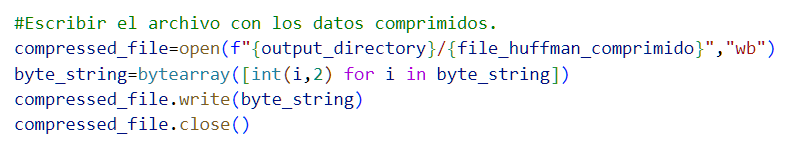
\includegraphics[width=0.9\linewidth]{figures/filehuffman.png}
  %      \caption{Función de lista en archivo binario usando file\_huffman\_comprimido}
 %       \label{fig:huffmanfile}
%    \end{center}
%\end{figure}

\begin{lstlisting}[language=Python, caption={Función de lista en archivo binario usando file\_huffman\_comprimido}, label={listing2}]
#Escribir el archivo con los datos comprimidos.
compressed_file=open(f"{output_directory}/{file_huffman_comprimido}","wb")
byte_string=bytearray([int(i,2) for i in byte_string])
compressed_file.write(byte_string)
compressed_file.close()
\end{lstlisting}

También se agregó una sección adicional de código cuya función es exportar los datos comprimidos en un archivo CSV. Este fragmento escribe tanto el tamaño comprimido en bits como cada par clave-valor del diccionario huffmanCode, registrando el símbolo y su correspondiente código Huffman. La Tabla \ref{tab:compression_stats}  muestra un resumen comparativo de los datos comprimidos obtenidos a partir de los archivos previamente utilizados.

\begin{table}[H]
    \centering
    \caption{Tamaño original, comprimido y tasa de compresión por archivo}
    \label{tab:compression_stats}
    \begin{tabular}{lccc}
        \toprule
        \textbf{Nombre del archivo} & \textbf{Tamaño Original (bytes)} & \textbf{Tamaño Comprimido (bytes)} & \textbf{Tasa de Compresión} \\
        \midrule
        todo\_ascii\_cien.bin & 25600  & 25600  & 1.00000 \\
        shannon\_intro.txt    & 7429   & 4085   & 1.81860 \\
        4.1.01.tiff 		  & 196748 & 170415 & 1.15452 \\
        4.2.03.tiff 		  & 786572 & 767063 & 1.02543 \\
        5.1.11.tiff			  & 65670  & 53196  & 1.23449 \\
        5.1.13.tiff 	   	  & 65670  & 16016  & 4.10027 \\
        7.1.02.tiff 		  & 262278 & 132955 & 1.97268 \\
        h\_cero.bin 		  & 1000   & 0      & - \\
        \bottomrule 
    \end{tabular}
\end{table}

Nótese que para el archivo "h\_cero.bin" no se muestra tasa de compresión, esto porque no hay diccionario de compresión al haber largo promedio igual a cero, lo que significa que todos los símbolos son iguales.

Al analizar resultados presentados en la Tabla \ref{tab:compression_stats} se puede evaluar la eficiencia del algoritmo de Huffman aplicado a archivos de textos y formatos de imagen TIFF.

En el caso del archivo todo\_ascii\_cien.bin, no se observa compresión alguna, ya que el tamaño original y el comprimido son idénticos. Esto nos dice que todos los símbolos tienen probabilidades similares. Según la teoría de codificación, cuando la distribución de probabilidad es uniforme, la codificación Huffman pierde su ventaja, ya que no puede asignar códigos más cortos a los símbolos más probables \cite{haykin}.

El archivo shannon\_intro.txt presenta una tasa de compresión cercana al 1.82, lo cual indica una compresión eficiente. Esta mejora se explica porque el texto posee una distribución de frecuencias sesgada, donde ciertas letras y espacios aparecen con  frecuencia. Tal como se discute en \cite{haykin}, este tipo de fuente tiene una entropía baja en relación al alfabeto completo, lo que permite que Huffman reduzca la longitud media del código por símbolo muy cerca del límite teórico de Shannon.

Para los archivos de imagen en formato TIFF, como 4.1.01.tiff o 4.2.03.tiff, se observa una compresión mucho más limitada. Esto puede deberse a que contienen patrones gráficos complejos.

En el archivo 5.1.13.tiff, se logra una tasa de compresión superior a 4.1. Este valor indica que la imagen en efecto tiene una estructura de datos con redundancias, lo cual reduce significativamente la entropía de la fuente. Por eso, Huffman se comporta de manera casi ideal asignando códigos muy cortos a los símbolos dominantes. Este fenómeno se alinea con la teoría de Shannon-Huffman que establece que, cuanto mayor sea la varianza entre las probabilidades de los símbolos, mayor será la ganancia de compresión \cite{haykin}.

Por otro lado, el archivo h\_cero.bin representa un caso límite de entropía nula, donde todos los símbolos son iguales. En ese escenario, como se deriva directamente de la definición de entropía, para un único símbolo, la entropía es cero y por tanto, no es necesario almacenar ningún dato aparte del símbolo mismo y su cantidad de repeticiones. Esto justifica que el archivo comprimido tenga un tamaño de cero bytes, ya que basta con almacenar una única referencia al símbolo repetido. 

Finalmente, archivos 7.1.02.tiff y 5.1.11.tiff, con tasas de compresión cercanas a 2 y 1.23 respectivamente, evidencian estructuras gráficas intermedias, donde la redundancia es presente pero no significativa. Lo que refleja una entropía moderada en los datos, permitiendo al algoritmo Huffman reducir el tamaño del archivo, pero no se observa una reducción tan notable.









\subsection{Restablecimiento de los datos originales - Descompresión}

\begin{lstlisting}[language=Python, caption={Código modificado para guardar los datos en una carpeta de destino}, label={listing3}]

#Abrir diccionario y descomprimir datos.
csvfile = open (f"{output_directory}/{ruta_diccionario}" , "r")
reader = csv . reader ( csvfile )
bits_a_leer = None 
diccionario = dict () 
for row in reader :
    if( bits_a_leer == None ) :
        bits_a_leer = int( row [0]) 
    else:
        diccionario.update ({ int( row [0]) : row [1]})
Decoding = NodeTree ( None , None ) 
for entrada in diccionario :
    insert_in_tree ( Decoding , diccionario [ entrada ] , entrada )
nodo = Decoding 
data_estimated = []
for i in range ( compressed_length_bit ) :
    (l , r ) = nodo . children () 
    if( binary_string [ i ]== "1") :
        nodo = r
    else:
        nodo = l
    if type ( nodo ) is int :
        data_estimated . append(nodo)
        nodo = Decoding


\end{lstlisting}

\textbf{¿Cuál es el propósito del código mostrado?}

Siguiendo el código en python tal cual, este tiene el propósito de ejecutar los siguientes pasos:

\begin{itemize}
\item Abrir un archivo en modo de lectura que tiene la ruta de almacenamiento en \texttt{ruta_diccionario}
\item Se crea una variable auxiliar \texttt{reader} que lee línea por línea el archivo csv.
\item Se inicializa la variable \texttt{bits_a_leer}
\item Se crea un diccionario vacío para guardar los datos decodificados
\item Se inicia la lectura del archivo csv con ayuda del reader, la primera fila del archivos se guardan en \texttt{bits_a_leer} y al terminar de guardarlos se actualizan las demás columnas en el diccionario.
\item Se crea un nuevo árbol binario.
\item Siguiendo iterativamente la entrada que corresponde al símbolo, se insertan en el árbol de decodificación.
\item Se inicializa las raíces del árbol de decodificación.
 \item Se inicializa una lista para guardar los datos decodificados
\item Se recorre sobre cada bit del string cuya longitud es \texttt{compressed_length_bit}.
\item Se obtiene los hijos izquierdo (l) y derecho (r) del nodo actual.
\item Se recorre a la izquierda o a la derecha dependiendo del bit actual ('0' o '1').
\item Se compara si el nodo actual es un entero (un nodo hoja), lo añade a \texttt{data_estimated}, y vuelve a la raíz para el siguiente símbolo.
\end{itemize}


En resumen, el código anterior consigue la decodificación siguiendo el árbol de Huff de arriba a hacia abajo rama a rama, hasta que se llega al nodo raíz. Dependiendo si se encuentra un 1 o 0, se recorre una rama u otra del árbol binario hasta que se llega al inicio y en consecuencia la palabra producto de las comparaciones genera la palabra de código fue codificada en un principio por el árbol binario.


\textbf{Comparación de datos estimados y los datos originales de la fuente}



\begin{table}[H]
\centering
\caption{Huffman Codigo 7.1.02.tiff}
\label{tab:compression_tiff}
\begin{tabular}{|c|c||c|c||c|c|}
\hline
\textbf{Char} & \textbf{Code} & \textbf{Char} & \textbf{Code} & \textbf{Char} & \textbf{Code} \\
\hline
177 & 100 & 180 & 011 & 175 & 010 \\
183 & 001 & 172 & 000 & 186 & 1111 \\
189 & 1101 & 192 & 1100 & 169 & 1010 \\
195 & 10110 & 167 & 111011 & 164 & 101110 \\
162 & 1110001 & 159 & 11100111 & 199 & 10111111 \\
157 & 10111110 & 155 & 111001101 & 49 & 111000001 \\
152 & 101111011 & 48 & 101111001 & 110 & 1110101101 \\
113 & 1110101100 & 112 & 1110101010 & 109 & 1110101000 \\
150 & 1110100101 & 115 & 1110100001 & 51 & 1110011000 \\
46 & 1110010111 & 117 & 1110010101 & 108 & 1110010011 \\
148 & 1110000111 & 118 & 1110000110 & 45 & 1110000100 \\
146 & 1110000000 & 106 & 1011110101 & 120 & 1011110100 \\
202 & 11101011111 & 47 & 11101011110 & 140 & 11101011100 \\
144 & 11101010111 & 130 & 11101010110 & 50 & 11101010010 \\
134 & 11101001111 & 53 & 11101001110 & 105 & 11101001100 \\
142 & 11101001001 & 138 & 11101001000 & 132 & 11101000111 \\
43 & 11101000110 & 55 & 11101000100 & 136 & 11101000001 \\
127 & 11101000000 & 121 & 11100110011 & 128 & 11100110010 \\
125 & 11100101101 & 123 & 11100101001 & 52 & 11100100100 \\
103 & 11100100010 & 42 & 10111100010 & 102 & 10111100001 \\
58 & 111010111010 & 101 & 111010100110 & 44 & 111001010001 \\
0 & 111001010000 & 41 & 111001001011 & 40 & 111001000110 \\
\hline
\end{tabular}
\end{table}


\begin{table}
\centering
\caption{Huffman Codigo 7.1.02_loss.jpeg}
\label{tab:compression_jpeg}
\begin{tabular}{|c|c||c|c||c|c|}
\hline
Char & Huffman Code & Char & Huffman Code & Char & Huffman Code \\
\hline
0 & 110001 & 231 & 0101000 & 255 & 0100010 \\
63 & 0100001 & 199 & 0100000 & 227 & 0011100 \\
219 & 0010100 & 249 & 0010010 & 207 & 0010001 \\
1 & 0001100 & 237 & 0001001 & 142 & 0001000 \\
113 & 0000111 & 243 & 0000110 & 3 & 0000100 \\
254 & 0000010 & 158 & 0000001 & 252 & 11111110 \\
110 & 11111101 & 31 & 11111100 & 7 & 11111010 \\
183 & 11111000 & 159 & 11110011 & 35 & 11110001 \\
127 & 11110000 & 79 & 11101111 & 218 & 11101101 \\
220 & 11101100 & 28 & 11101001 & 115 & 11100111 \\
235 & 11100110 & 126 & 11100101 & 242 & 11100100 \\
221 & 11100011 & 187 & 11100010 & 145 & 11100001 \\
57 & 11100000 & 143 & 11011111 & 64 & 11011110 \\
99 & 11011100 & 60 & 11011011 & 128 & 11011010 \\
61 & 11011001 & 12 & 11011000 & 238 & 11010111 \\
122 & 11010110 & 109 & 11010101 & 251 & 11010100 \\
156 & 11010011 & 29 & 11010010 & 85 & 11010001 \\
25 & 11001111 & 56 & 11001110 & 167 & 11001101 \\
211 & 11001100 & 62 & 11001010 & 233 & 11001001 \\
140 & 11001000 & 149 & 11000011 & 250 & 11000010 \\
223 & 11000001 & 120 & 11000000 & 118 & 10111111 \\
59 & 10111110 & 184 & 10111101 & 230 & 10111100 \\
\hline
\end{tabular}
\end{table}

Seguidamente, al correr el script para cada caso la codificación óptima visitante se puede comprobar en las Tabla \ref{tab:compression_jpeg} y la Tabla \ref{tab:compression_tiff}. Y para corroborar el código recuperado en los anexos se describen las Tabla \ref{tab:dict_compact1} y Tabla \ref{tab:loss_dict_compact} con los datos obtenidos.

La forma de decodificación que se plantea es por medio del seguimiento bit a bit del Árbol de Huffman, consiguiendo un resultado rápido de la palabra que se codificó. Sin embargo, en casos que la fuente conste de símbolos muy grandes la computación aumenta y por ende tanto los recursos como el tiempo de ejecución de la codificación se puede volver impráctica si hay limitantes como los mencionados.










\subsection{Efecto de la entropía de la fuente}
\textbf{¿Qué diferencias hay entre ellos? }

\begin{table}[h!]
    \centering
    \caption{Comparación misma imagen con distinto formato }
    \label{tab:jpeg_vs_tiff}
    \begin{tabular}{cccc}
    \toprule
    \textbf{Tipo} & \textbf{Tamaño} & \textbf{Ancho} & \textbf{Largo} \\
    \midrule
    Imagen JPEG & 59.3 kB (59,323 bytes) & 512 pixels & 512 pixels \\
    Imagen TIFF & 262.3 kB(262,278 bytes)& 512 pixels & 512 pixels \\
    \bottomrule
    \end{tabular}
\end{table}


Al revisar las propiedades de ambos  archivos se puede constatar que para el caso del archivo .tiff tiene un mayor tamaño en comparación del archivo .jpeg, según la Tabla. \ref{tab:jpeg_vs_tiff}, esto se puede ver como que .tiff es aproximadamente es 5 veces el tamaño de .jpeg. Esa gran diferencia tiene sentido dado que en la teoría la diferencia entre estos dos tipicamente se distinguen por la compresión que se refleja en el tamaño y calidad de las imágenes, para el caso del formato JPEG utiliza compresión con pérdidas y el caso TIFF utiliza compresión sin pérdidas.


\textbf{Formato JPEG}

JPEG por sus siglas de Joint Photographic Experts Group (Grupo Conjunto de Expertos en Fotografía), fue una organización internacional que estandarizó el formato a finales de los ochenta y principios de los noventa. Es el formato de archivo preferido para las imágenes digitales, y lo ha sido desde que los fotógrafos empezaron a capturar y almacenar imágenes en cámaras digitales y otros dispositivos reprográficos \cite{balanis}.

Las imágenes JPEG agrupan las siguientes extensiones de nombre de archivo:

\begin{itemize}
\item .jpg
\item .jpeg
\item .jpe
\item .jif
\item .jfif
\item .jfi
\end{itemize}


Un archivo JPEG admite hasta 24 bits de color y utiliza compresión con pérdida para comprimir las imágenes y facilitar su almacenamiento y envío. Esto puede hacer que los JPEG sean mejores para el uso diario, pero implica sacrificar parte de la calidad de la imagen original.


\textbf{Formato TIFF}

Un TIFF(Tag Image File Format) es un archivo informático utilizado para almacenar gráficos rasterizados e información de imágenes. Los TIFF, favoritos de los fotógrafos, son una forma práctica de almacenar imágenes de alta calidad antes de editarlas si quieres evitar los formatos de archivo con pérdidas.

Archivos TIFF:
\begin{itemize}
\item Tienen extensión .tiff o .tif.
\item Son una forma de compresión de archivos sin pérdidas, lo que significa que son más grandes que la mayoría pero no pierden calidad de imagen.
\item Los TIFF no son los archivos más pequeños que existen, pero permiten al usuario etiquetar información y datos adicionales de la imagen, como capas adicionales.
\end{itemize}




\textbf{¿Qué diferencias ve en los resultados? ¿Porqué se da un cambio tan grande?}
\begin{table}[H]
    \centering
    \caption{Tamaño original, comprimido y tasa de compresión por archivo}
    \label{tab:compression_same}
    \begin{tabular}{lcccc}
        \toprule
        \textbf{Nombre del archivo} & \textbf{Entropia de la fuente$H(\Sigma)$}& \textbf{Varianza código original ($\sigma^2$ )} & \textbf{Tamaño Comprimido (bytes)} & \textbf{Tasa de Compresión} \\
        \midrule
        7.1.02_loss.jpg & 7.93548& 0.260 &59033  & 1.004912 \\
        7.1.02.tiff 	& 4.00 & 3.68  &  132955 & 1.97268 \\
        \bottomrule 
    \end{tabular}
\end{table}


Al correr el script en cada caso se obtienen los datos recabados de la Tabla \ref{tab:compression_same}, se puede ver que el tamaño del archivo .tiff tuvo una disminución considerable más de 100 mil bytes respecto al archivo original con una tasa de 1.97268, mientras que para el caso con pérdidas la disminución respecto al archivo original fue cercano a los 300 bytes con una tasa de prácticamente igual a la unidad.

Analizando las respuestas de ambos archivos, se pueden encontrar factores claves del por qué la relación de compresión entre ambos archivos no es similar y esto se debe a parámetros que se enlistan la Tabla \ref{tab:compression_same}, basados en la teoría de la información. El principal parámetro que produce un cambio en la compresión es la varianza, que en términos simples entre mayor sea este valor los datos están más dispersos y por ende hay mayor probabilidad de disminuir el espacio entre ellos sin perder información, es decir, hay una mayor presencia de redundancia que se puede optimizar y en consecuencia reducir el tamaño del archivo.

Recordando la teoría otra medida relevante es la entropía de la fuente, que indica el nivel de incertidumbre y refleja que a mayor su valor los símbolos que se transmiten tienen más informacion.
\section{Conclusiones} 

\begin{itemize}

\item Se comprobó 

\item El 

\item Se demostró 

\item  En cuanto

\end{itemize}


\section{Referencias Bibliográficas}
\printbibliography[heading=none]

\section{Anexos}
Datos recuperados para cada archivo solicitado inciso 2.4 .

\begin{table}[h]
\centering
\caption{Diccionario de 7.1.02$\_diccionario.csv$}
\label{tab:dict_compact1}
\begin{tabular}{cccccc}
\hline
\textbf{Value} & \textbf{Code} & \textbf{Value} & \textbf{Code} & \textbf{Value} & \textbf{Code} \\ \hline
172 & 000 & 183 & 001 & 175 & 010 \\ \hline
180 & 011 & 177 & 100 & 169 & 1010 \\ \hline
195 & 10110 & 164 & 101110 & 38 & 101111000000 \\ \hline
72 & 1011110000010 & 73 & 1011110000011 & 102 & 10111100001 \\ \hline
42 & 10111100010 & 77 & 1011110001100 & 63 & 1011110001101 \\ \hline
97 & 101111000111 & 48 & 101111001 & 120 & 1011110100 \\ \hline
106 & 1011110101 & 152 & 101111011 & 157 & 10111110 \\ \hline
199 & 10111111 & 192 & 1100 & 189 & 1101 \\ \hline
146 & 1110000000 & 86 & 1110000001000 & 84 & 1110000001001 \\ \hline
99 & 111000000101 & 245 & 111000000110000000 & 236 & 111000000110000001 \\ \hline
10 & 111000000110000010 & 250 & 111000000110000011 & 31 & 111000000110000100 \\ \hline
26 & 111000000110000101 & 241 & 111000000110000110 & 228 & 111000000110000111 \\ \hline
220 & 11100000011000100 & 28 & 11100000011000101 & 6 & 111000000110001100 \\ \hline
254 & 111000000110001101 & 21 & 111000000110001110 & 17 & 111000000110001111 \\ \hline
29 & 1110000001100100 & 224 & 11100000011001010 & 232 & 111000000110010110 \\ \hline
22 & 1110000001100101110 & 20 & 1110000001100101111 & 3 & 111000000110011 \\ \hline
85 & 1110000001101 & 66 & 1110000001110 & 90 & 1110000001111 \\ \hline
49 & 111000001 & 45 & 1110000100 & 94 & 111000010100 \\ \hline
61 & 111000010101 & 56 & 111000010110 & 57 & 111000010111 \\ \hline
118 & 1110000110 & 148 & 1110000111 & 162 & 1110001 \\ \hline
65 & 111001000000 & 69 & 1110010000010 & 75 & 11100100000110 \\ \hline
74 & 11100100000111 & 87 & 1110010000100 & 67 & 1110010000101 \\ \hline
54 & 111001000011 & 103 & 11100100010 & 40 & 111001000110 \\ \hline
79 & 1110010001110 & 91 & 1110010001111 & 52 & 11100100100 \\ \hline
88 & 1110010010100 & 60 & 1110010010101 & 41 & 111001001011 \\ \hline
108 & 1110010011 & 0 & 111001010000 & 44 & 111001010001 \\ \hline
123 & 11100101001 & 117 & 1110010101 & 92 & 1110010110000 \\ \hline
70 & 1110010110001 & 78 & 11100101100100 & 4 & 1110010110010100 \\ \hline
25 & 11100101100101010 & 24 & 11100101100101011 & 2 & 11100101100101100 \\ \hline
216 & 11100101100101101 & 32 & 1110010110010111 & 39 & 11100101100110 \\ \hline
80 & 11100101100111 & 125 & 11100101101 & 46 & 1110010111 \\ \hline
51 & 1110011000 & 128 & 11100110010 & 121 & 11100110011 \\ \hline
155 & 111001101 & 159 & 11100111 & 127 & 11101000000 \\ \hline
136 & 11101000001 & 115 & 1110100001 & 55 & 11101000100 \\ \hline
59 & 1110100010100 & 76 & 11101000101010 & 205 & 11101000101011 \\ \hline
33 & 111010001011000 & 34 & 111010001011001 & 1 & 11101000101101 \\ \hline
93 & 1110100010111 & 43 & 11101000110 & 132 & 11101000111 \\ \hline
138 & 11101001000 & 142 & 11101001001 & 150 & 1110100101 \\ \hline
105 & 11101001100 & 68 & 11101001101000 & 71 & 11101001101001 \\ \hline
35 & 11101001101010 & 36 & 11101001101011 & 96 & 1110100110110 \\ \hline
98 & 1110100110111 & 53 & 11101001110 & 134 & 11101001111 \\ \hline
109 & 1110101000 & 50 & 11101010010 & 101 & 111010100110 \\ \hline
81 & 11101010011100 & 82 & 11101010011101 & 37 & 1110101001111 \\ \hline
112 & 1110101010 & 130 & 11101010110 & 144 & 11101010111 \\ \hline
113 & 1110101100 & 110 & 1110101101 & 140 & 11101011100 \\ \hline
58 & 111010111010 & 62 & 11101011101100 & 30 & 1110101110110100 \\ \hline
8 & 11101011101101010 & 27 & 111010111011010110 & 23 & 111010111011010111 \\ \hline
213 & 1110101110110110 & 209 & 1110101110110111 & 83 & 11101011101110 \\ \hline
64 & 11101011101111 & 47 & 11101011110 & 202 & 11101011111 \\ \hline
167 & 111011 & 186 & 1111 &  &  \\ \hline
\end{tabular}
\end{table}








\begin{table}[h]
\centering
\caption{Diccionario de 7.1.02$\_loss\_diccionario.csv$}
\label{tab:loss_dict_compact}
\begin{tabular}{cccccc}
\hline
\textbf{Value} & \textbf{Code} & \textbf{Value} & \textbf{Code} & \textbf{Value} & \textbf{Code} \\ \hline
148 & 00000000 & 67 & 00000001 & 158 & 0000001 \\ \hline
254 & 0000010 & 74 & 00000110 & 93 & 00000111 \\ \hline
3 & 0000100 & 213 & 00001010 & 82 & 00001011 \\ \hline
243 & 0000110 & 113 & 0000111 & 142 & 0001000 \\ \hline
237 & 0001001 & 65 & 00010100 & 152 & 00010101 \\ \hline
236 & 00010110 & 69 & 00010111 & 1 & 0001100 \\ \hline
53 & 00011010 & 193 & 00011011 & 166 & 00011100 \\ \hline
96 & 00011101 & 45 & 00011110 & 178 & 00011111 \\ \hline
48 & 00100000 & 226 & 00100001 & 207 & 0010001 \\ \hline
249 & 0010010 & 98 & 00100110 & 216 & 00100111 \\ \hline
219 & 0010100 & 116 & 00101010 & 43 & 00101011 \\ \hline
138 & 00101100 & 131 & 00101101 & 144 & 00101110 \\ \hline
234 & 00101111 & 20 & 00110000 & 47 & 00110001 \\ \hline
217 & 00110010 & 55 & 00110011 & 40 & 00110100 \\ \hline
117 & 00110101 & 108 & 00110110 & 186 & 00110111 \\ \hline
227 & 0011100 & 5 & 00111010 & 197 & 00111011 \\ \hline
58 & 00111100 & 11 & 00111101 & 6 & 00111110 \\ \hline
200 & 00111111 & 199 & 0100000 & 63 & 0100001 \\ \hline
255 & 0100010 & 151 & 01000110 & 94 & 01000111 \\ \hline
164 & 01001000 & 153 & 01001001 & 89 & 01001010 \\ \hline
77 & 01001011 & 190 & 01001100 & 101 & 01001101 \\ \hline
100 & 01001110 & 133 & 01001111 & 231 & 0101000 \\ \hline
90 & 01010010 & 174 & 01010011 & 212 & 01010100 \\ \hline
192 & 01010101 & 92 & 01010110 & 86 & 01010111 \\ \hline
165 & 01011000 & 163 & 01011001 & 134 & 01011010 \\ \hline
44 & 01011011 & 21 & 01011100 & 88 & 01011101 \\ \hline
83 & 01011110 & 72 & 01011111 & 246 & 01100000 \\ \hline
177 & 01100001 & 4 & 01100010 & 228 & 01100011 \\ \hline
91 & 01100100 & 105 & 01100101 & 162 & 011001100 \\ \hline
132 & 011001101 & 104 & 01100111 & 130 & 01101000 \\ \hline
150 & 01101001 & 87 & 01101010 & 14 & 01101011 \\ \hline
244 & 01101100 & 210 & 01101101 & 103 & 01101110 \\ \hline
172 & 01101111 & 50 & 01110000 & 202 & 01110001 \\ \hline
179 & 01110010 & 52 & 01110011 & 102 & 01110100 \\ \hline
10 & 01110101 & 39 & 01110110 & 240 & 01110111 \\ \hline
95 & 01111000 & 141 & 01111001 & 189 & 01111010 \\ \hline
112 & 01111011 & 225 & 01111100 & 155 & 01111101 \\ \hline
204 & 01111110 & 188 & 01111111 & 214 & 10000000 \\ \hline
2 & 10000001 & 80 & 10000010 & 171 & 10000011 \\ \hline
208 & 10000100 & 78 & 10000101 & 124 & 10000110 \\ \hline
203 & 10000111 & 182 & 10001000 & 147 & 10001001 \\ \hline
215 & 10001010 & 168 & 10001011 & 16 & 100011000 \\ \hline
68 & 100011001 & 30 & 10001101 & 54 & 10001110 \\ \hline
27 & 10001111 & 49 & 10010000 & 123 & 10010001 \\ \hline
51 & 10010010 & 205 & 10010011 & 239 & 10010100 \\ \hline
121 & 10010101 & 24 & 10010110 & 73 & 10010111 \\ \hline
224 & 10011000 & 241 & 10011001 & 195 & 10011010 \\ \hline
119 & 10011011 & 173 & 10011100 & 248 & 10011101 \\ \hline
125 & 10011110 & 111 & 10011111 & 222 & 10100000 \\ \hline
66 & 101000010 & 33 & 101000011 & 84 & 10100010 \\ \hline
70 & 10100011 & 180 & 10100100 & 201 & 10100101 \\ \hline
114 & 10100110 & 36 & 10100111 & 185 & 10101000 \\ \hline
146 & 10101001 & 191 & 10101010 & 206 & 10101011 \\ \hline
71 & 10101100 & 253 & 10101101 & 170 & 10101110 \\ \hline
15 & 10101111 & 160 & 10110000 & 229 & 10110001 \\ \hline
181 & 10110010 & 175 & 10110011 & 42 & 10110100 \\ \hline
245 & 10110101 & 198 & 10110110 & 169 & 10110111 \\ \hline
19 & 101110000 & 136 & 101110001 & 106 & 10111001 \\ \hline
247 & 10111010 & 154 & 10111011 & 230 & 10111100 \\ \hline
184 & 10111101 & 59 & 10111110 & 118 & 10111111 \\ \hline
120 & 11000000 & 223 & 11000001 & 250 & 11000010 \\ \hline
149 & 11000011 & 0 & 110001 & 140 & 11001000 \\ \hline
233 & 11001001 & 62 & 11001010 & 23 & 110010110 \\ \hline
137 & 110010111 & 211 & 11001100 & 167 & 11001101 \\ \hline
56 & 11001110 & 25 & 11001111 & 209 & 110100000 \\ \hline
37 & 110100001 & 85 & 11010001 & 29 & 11010010 \\ \hline
156 & 11010011 & 251 & 11010100 & 109 & 11010101 \\ \hline
122 & 11010110 & 238 & 11010111 & 12 & 11011000 \\ \hline
61 & 11011001 & 128 & 11011010 & 60 & 11011011 \\ \hline
99 & 11011100 & 22 & 110111010 & 194 & 110111011 \\ \hline
64 & 11011110 & 143 & 11011111 & 57 & 11100000 \\ \hline
145 & 11100001 & 187 & 11100010 & 221 & 11100011 \\ \hline
242 & 11100100 & 126 & 11100101 & 235 & 11100110 \\ \hline
115 & 11100111 & 81 & 111010000 & 13 & 111010001 \\ \hline
28 & 11101001 & 8 & 111010100 & 41 & 111010101 \\ \hline
34 & 111010110 & 46 & 111010111 & 220 & 11101100 \\ \hline
218 & 11101101 & 97 & 111011100 & 75 & 111011101 \\ \hline
79 & 11101111 & 127 & 11110000 & 35 & 11110001 \\ \hline
17 & 111100100 & 129 & 111100101 & 159 & 11110011 \\ \hline
38 & 111101000 & 196 & 111101001 & 18 & 111101010 \\ \hline
139 & 111101011 & 176 & 111101100 & 161 & 111101101 \\ \hline
9 & 111101110 & 135 & 111101111 & 183 & 11111000 \\ \hline
76 & 111110010 & 107 & 111110011 & 7 & 11111010 \\ \hline
26 & 111110110 & 157 & 111110111 & 31 & 11111100 \\ \hline
110 & 11111101 & 252 & 11111110 & 32 & 111111110 \\ \hline
232 & 111111111 &  &  &  &  \\ \hline
\end{tabular}
\end{table}







\href{https://github.com/NagelMS/Tarea2_CE2.git}{Link al repositorio de GitHub}

\end{document} 

 

 

 
